\begin{figure}[t]
    \centering
    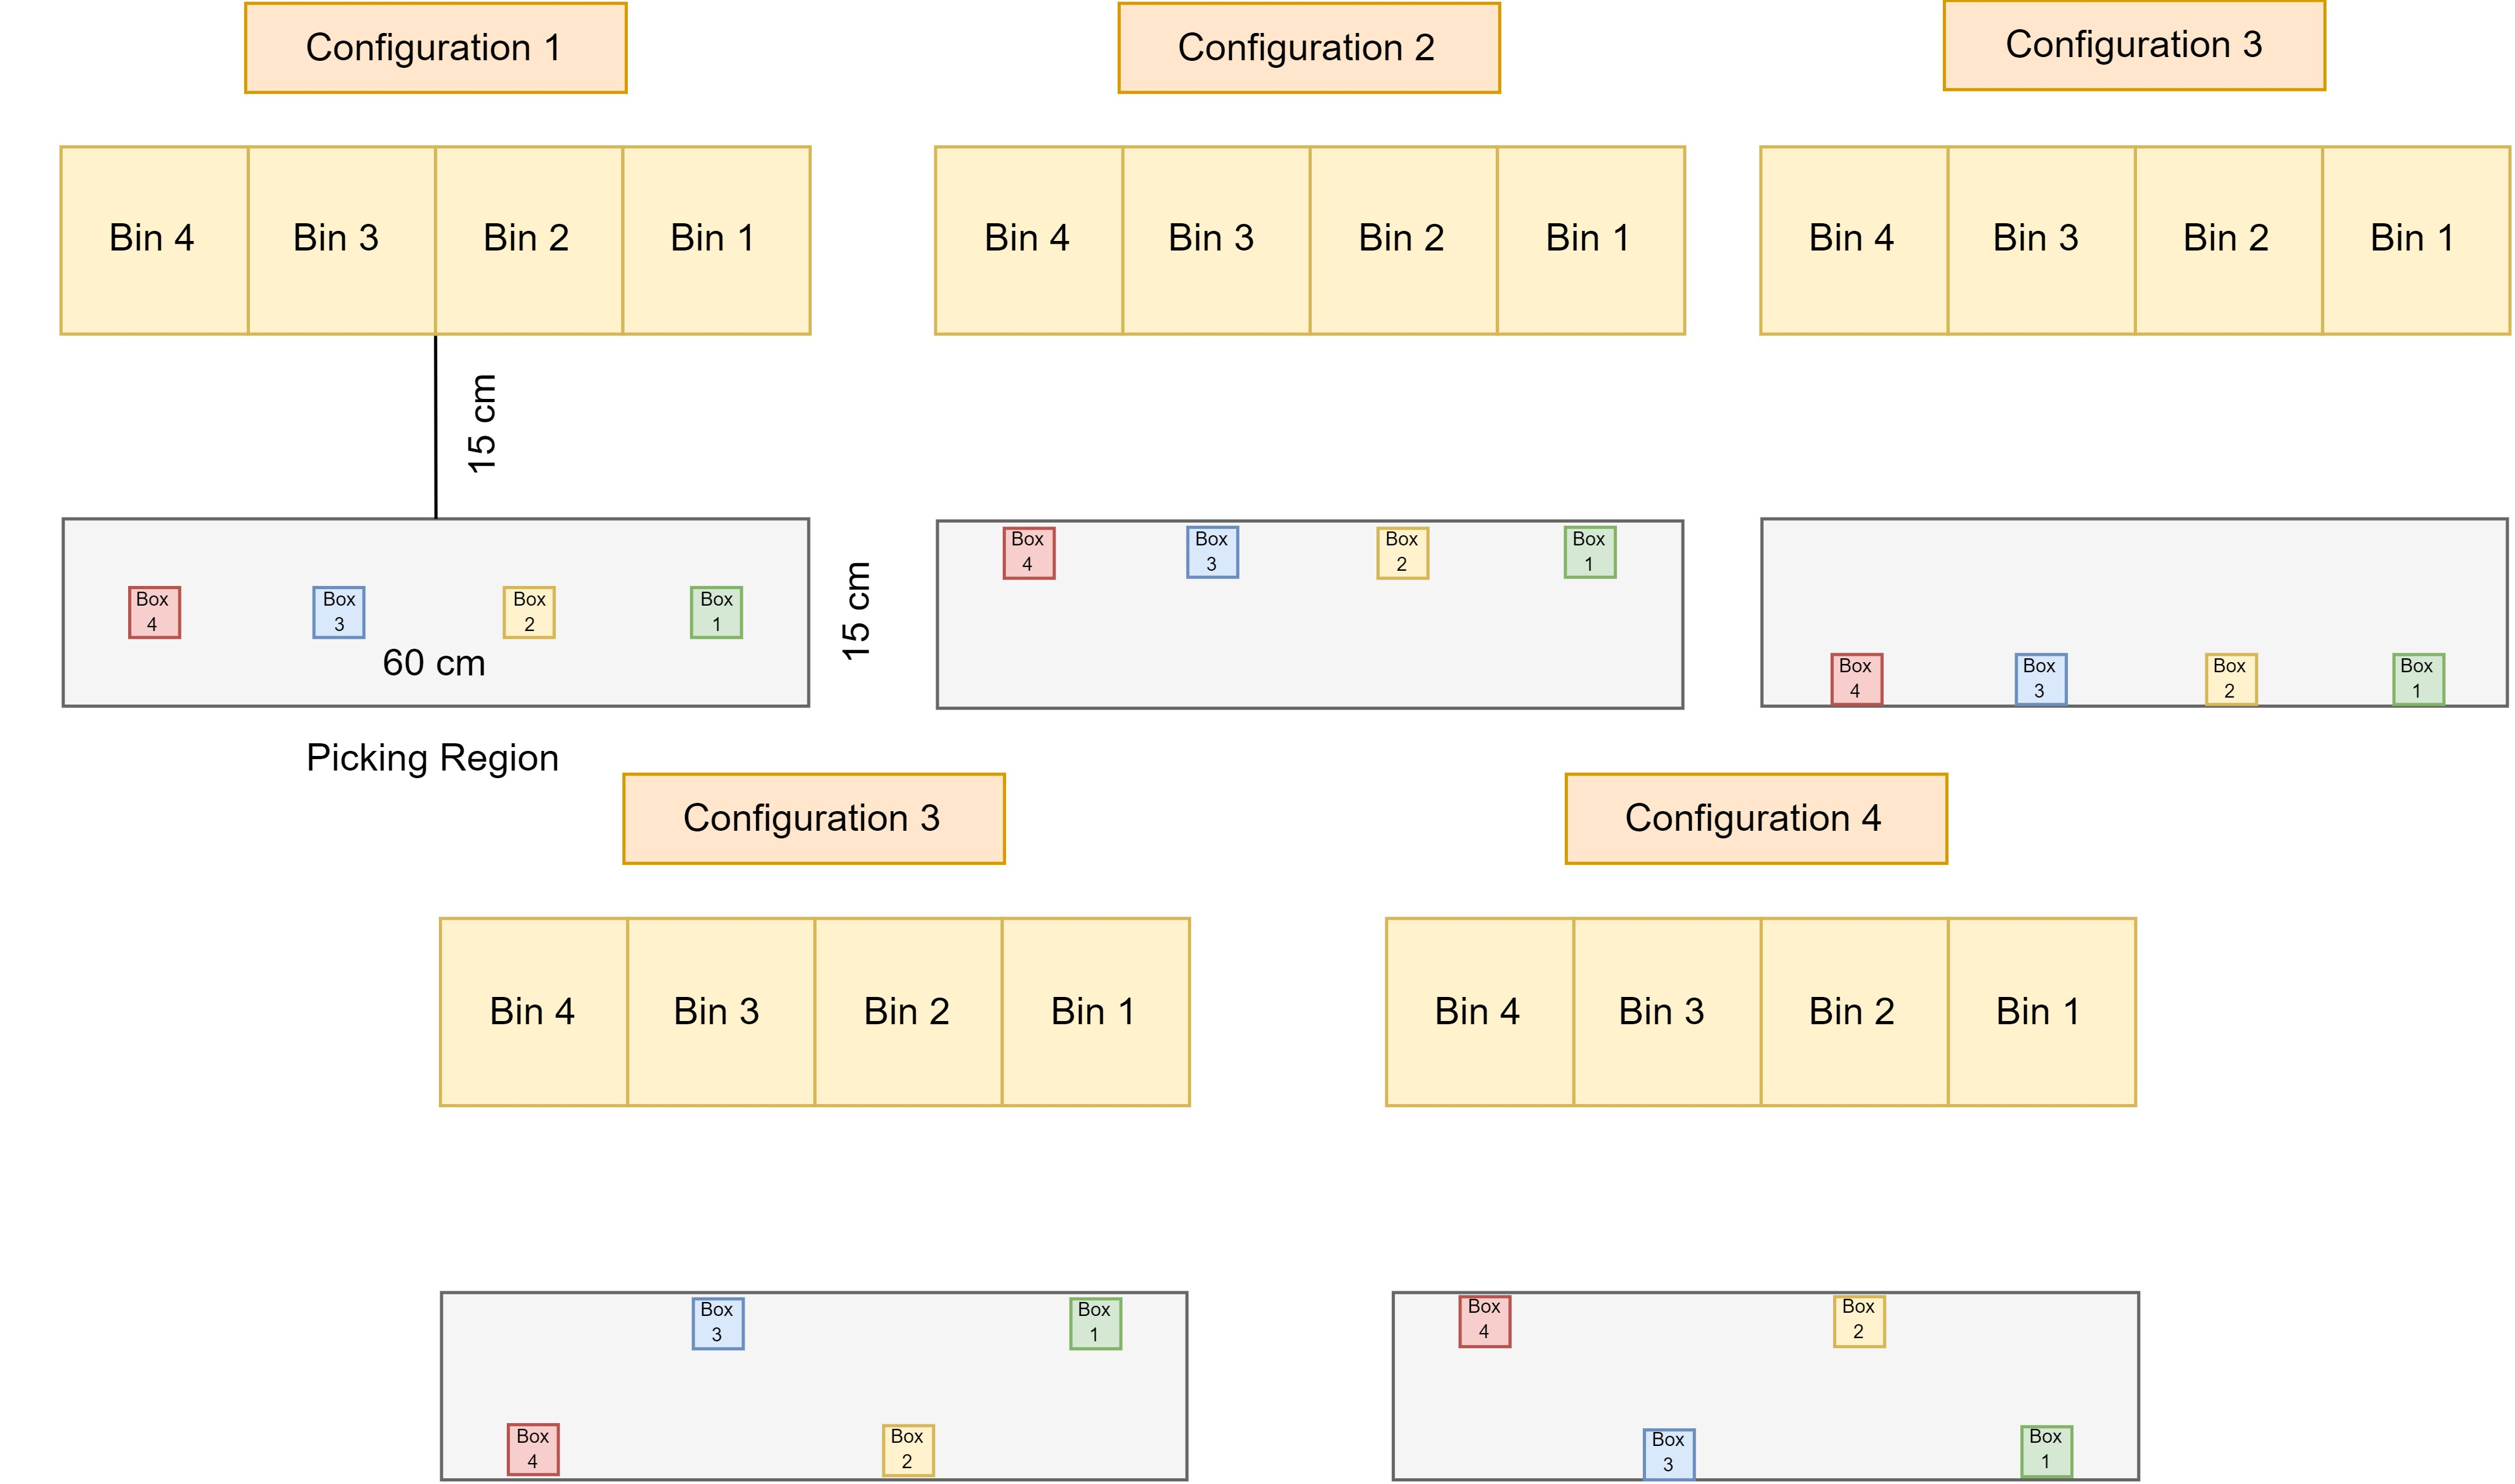
\includegraphics[width=0.8\textwidth]{figures/images/ch5/box_placement.jpg}
    \caption{Placement configuration used for the trajectory collection. For each placement configuration, 4 trajectories were collected. The target object initially starts at the rightmost position, and in each subsequent trajectory, the box is moved to the adjacent position. This process is then repeated twice, each time with a different object orientation, resulting in a total of 40 trajectories for a given configuration.}
    \label{fig:box_placement}
\end{figure}
